% !TEX program = xelatex

\documentclass[11pt]{padajar-memo}

% Required document information
\name         {paolo adajar}
\email        {paoloadajar@mit.edu}
\memonote	  {v1.0.0}					% in practice, often used for who the note is going to
\date         {\today}
\pdftitle     {test}

\memotitle{padajar-templates}

\newcommand{\ttslash}[1]{\texttt{\textbackslash #1}}
\usepackage{array}   % for \newcolumntype macro
\newcolumntype{T}{>{\ttfamily}p{1.75in}} % teletype version of "l" column type

\setlength\textfloatsep{0pt}
\setlength\belowcaptionskip{0pt}
\captionsetup[figure]{skip=0pt}
\setlength\fboxsep{0pt}

\begin{document}

\section*{about}

\texttt{padajar-templates} is a series of \LaTeX{} classes made by Paolo Adajar (that's me!). This originated as a series of \LaTeX{} commands in summer 2021, used just for psets, but has since transformed into several classes (\texttt{padajar-memo}, \texttt{padajar-pset}, and \texttt{padajar-slides}) relying on a common package (\texttt{padajar-defaults}). I'm hoping the up-front cost of creating them will be paid back many times over in my future work, and that of others.

These files are open-source and distributed under an MIT License (see \Cref{license}). If you do use them, I greatly appreciate:
\begin{itemize}
	\item hearing about it
	\item attribution
	\item contributing, if that's up your alley
	\item spreading the word!
\end{itemize}

\renewcommand{\contentsname}{contents}
\tableofcontents

\clearpage

\section{padajar-defaults}
All \texttt{padajar-templates} load the package \texttt{padajar-defaults}. This package comes with the following features/options.

\begin{itemize}
	\item Body and math font set to IBM Plex. Body text is IBM Plex Sans by default, but can be changed with the \texttt{[serif]} option to IBM Plex Serif. Math font is always serif, like $\sin^2(\alpha) + \cos^2(\alpha) = 1$ and
	\[
	\Phi(x) = \int_{-\infty}^x \frac{e^{-t^2/2}}{\sqrt{2\pi}} \dd{t}.
	\]
	Mono font is set to IBM Plex Mono. All fonts are set to user a lighter weight than the default.

	Note that because the \texttt{fontspec} package is used, to use this package (and any below templates), \textbf{you must} use XeLaTeX or LuaLaTeX. (For me, compilation with the former has been slightly faster.)
	\item A host of packages loaded by default:
	\begin{itemize}
		\item for math: \texttt{amsmath}, \texttt{amsthm}, \texttt{physics}, \texttt{bbm}\dots
		\item for graphics: \texttt{graphicx}, \texttt{pdfpages}, \texttt{listings}\dots
		\item for tables: \texttt{tabularx}, \texttt{booktabs}, \texttt{threeparttable}\dots
		\item for general utility: \texttt{hyperref}, \texttt{cleveref}, \texttt{enumitem}, \texttt{xcolor}\dots
	\end{itemize}
	If you want the full list, head into the source code of this package.
	\item A \texttt{listings} definition for Stata (modified from \href{https://github.com/satejsoman/stata-lstlisting}{here}), along with a nicer \texttt{listings} scheme.
	\item Some math commands I find useful: \ttslash{eps} ($\eps$), \ttslash{E} ($\E$), \ttslash{V} ($\V$), and \ttslash{indic} ($\indic$).
	\item A \texttt{padajar} color scheme! :)
\end{itemize}

A few other options are used internally by the classes to differentiate between documents and slides.

Notably, \texttt{padajar-defaults} is a standalone package. It can be used in any document, not just those in \texttt{padajar-templates}, granting additional flexibility.

\section{classes}

I've made three different formats that use \texttt{padajar-defaults}, each with its own purpose. These cover the vast majority of things that I create: paragraph-dense writing, problem sets, and presentation slides. I've put the same design ethos through them (and my website), with the intent of making my digital presence a tad more ``cohesive''.

\subsection{padajar-memo}
This is the simplest template of the three, and is the one that you're currently viewing.

\begin{figure}[ht]
	\caption{A preview of the \texttt{padajar-memo} class from \texttt{memo-example.pdf.}}
	\begin{center}
		\fbox{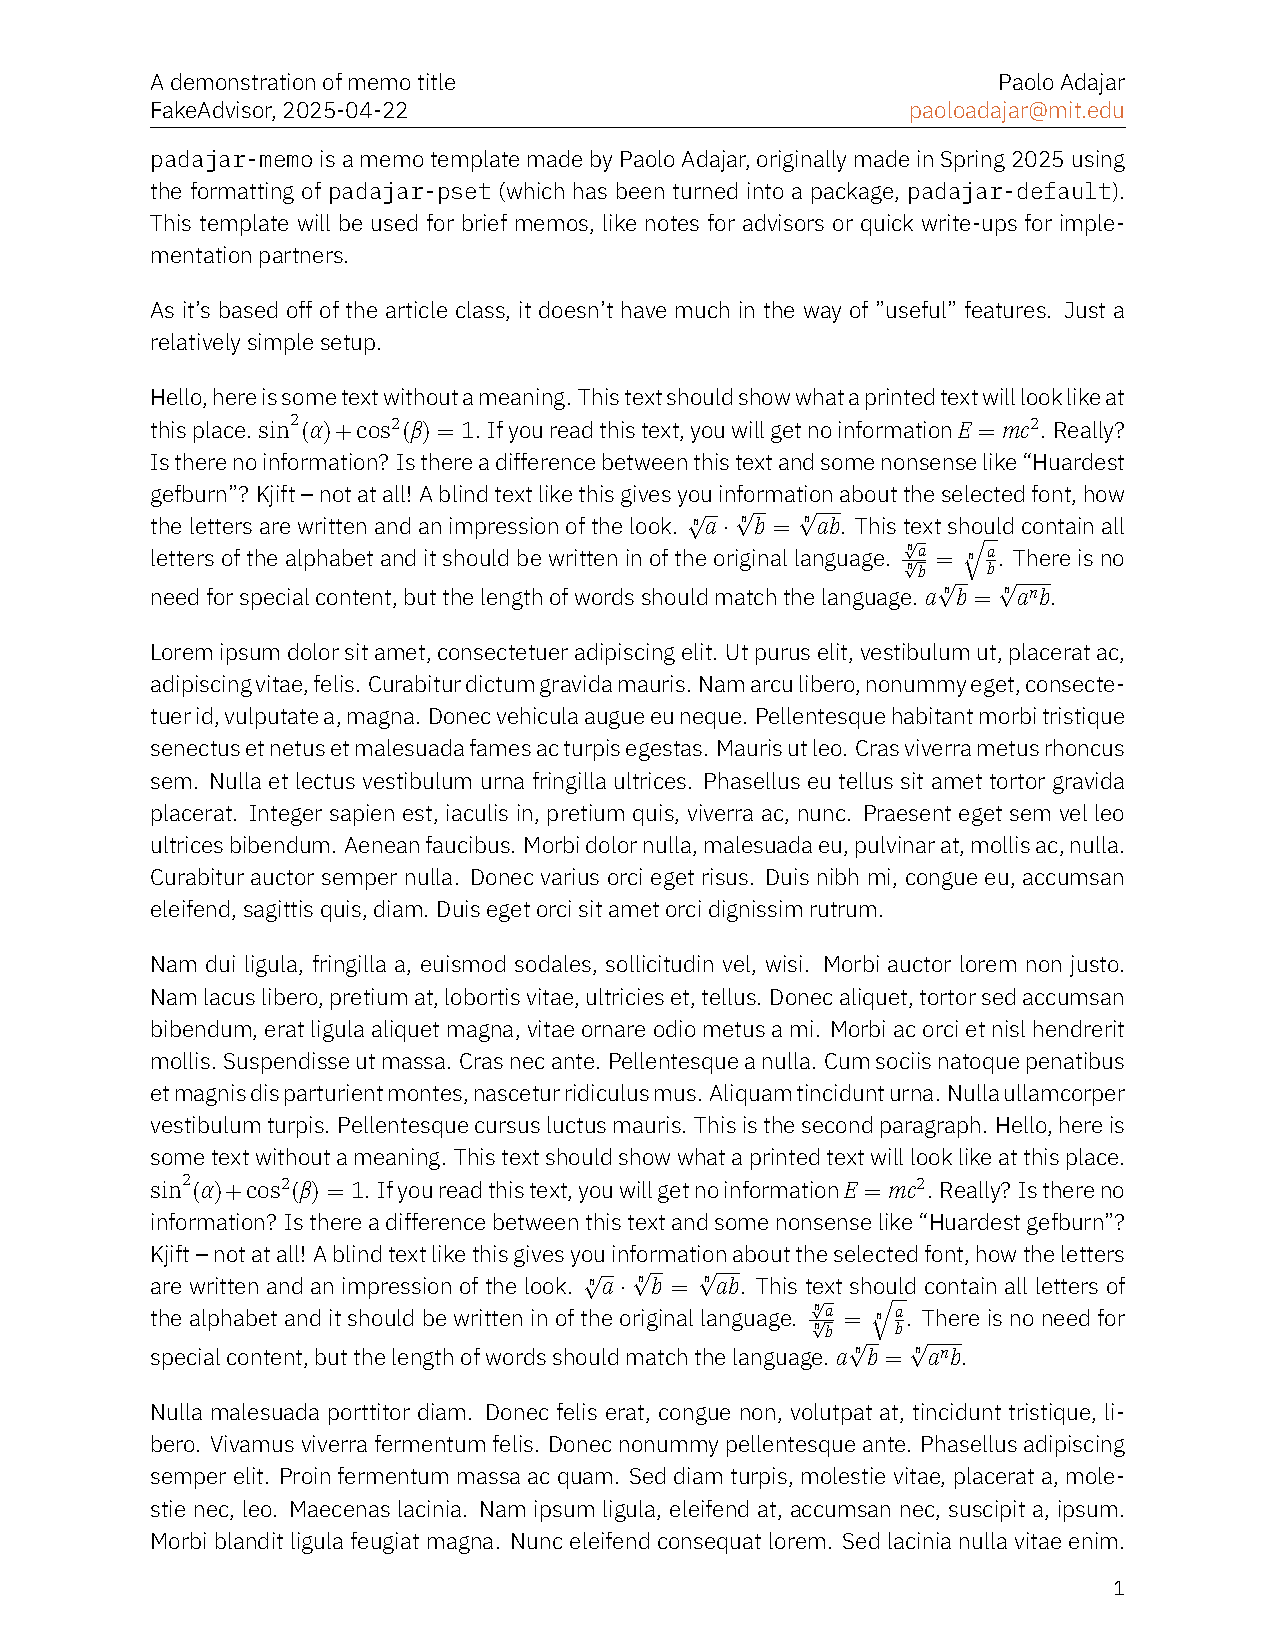
\includegraphics[width=0.48\textwidth,page=1]{memo/memo-example.pdf}}
		\fbox{\includegraphics[width=0.48\textwidth,page=2]{memo/memo-example.pdf}}
	\end{center}
\end{figure}


\texttt{padajar-memo} is intended for ideas that are communicated with paragraphs, tables, and figures. At its core, it's really just an \texttt{article} document with my usual settings. It comes with these additional features:

\begin{itemize}
	\item Fancy headers and footers, which take information from \ttslash{name}, \ttslash{email}, \ttslash{date}, \ttslash{memotitle}, and \ttslash{memonote}.
\end{itemize}

\dots and that's really it. The base setup of this class isn't too far different from the \texttt{article} class. It's just meant to be a clean baseline template so I don't always have to futz around with the same imports and options that I always do.

\subsection{padajar-pset}
This class is meant for writing up psets or exams with solutions. As a modification of the \texttt{exam} class, it retains all \texttt{exam} class functionality, like \texttt{parts} and \texttt{subparts}, the \texttt{solution} environment, and creating versions with and without answers included. For more information, refer to \href{https://www.overleaf.com/learn/latex/Typesetting\_exams\_in\_LaTeX}{this Overleaf page}.

\begin{figure}[ht]
	\caption{A preview of the \texttt{padajar-memo} class from \texttt{pset-example.pdf.}}
	\begin{center}
	\fbox{\includegraphics[width=0.48\textwidth,page=4]{pset/pset-example.pdf}}
	\fbox{\includegraphics[width=0.48\textwidth,page=5]{pset/pset-example.pdf}}
	\end{center}
\end{figure}

Some key features I've added in:
\begin{itemize}
	\item The \texttt{reflection} environment. These question reflections are intended to help connect questions to the course as a whole, interesting insights gained through the question, and more. Really, they're just a way to help think more about the ``why" of questions. These are encased in a gray \texttt{colorbox}, and can be included either by passing the \texttt{reflections} option to the class or adding \texttt{printreflections} to the preamble.

	\item The \texttt{solution} environment is encased in a green \texttt{tcolorbox}.

	\item Headers and footers which take information from \ttslash{name}, \ttslash{email}, \ttslash{date}, \ttslash{date}, \ttslash{classnum}, \ttslash{classname}, and \ttslash{assignment}. Optionally, \ttslash{professors} and \ttslash{collaborators} can take infinite arguments (separated with curly brackets) and add that information to the first page.
\end{itemize}

And some usage notes:

\begin{itemize}
	\item Questions are styled like sections; you should use \ttslash{titledquestion} command for creating questions, and \textit{then} write your question text (i.e., not in the question title). While I know this won't work for every field, multi-part questions are the bread and butter of economics psets.
	\item You can't use \texttt{table} environment (or any other \texttt{float} environment) inside the \texttt{solution} environment. This is currently solved using the \texttt{float} package, and then using the command \ttslash{begin\{table\}[H]}. I'm still looking for a ``better" solution to this.
\end{itemize}

\subsection{padajar-slides}
This class is based on the \texttt{moloch} theme for the \texttt{beamer} class, hosted on CTAN \href{https://ctan.org/pkg/moloch}{here}.\footnote{\texttt{moloch} itself is a fork of the \texttt{metropolis} theme, hosted on CTAN \href{https://ctan.org/pkg/beamertheme-metropolis}{here}. \texttt{metropolis} is no longer maintained, and \texttt{moloch} was created to fix some of its bugs --- see \href{https://jolars.co/blog/2024-05-30-moloch/}{this blog post}.} These are used for presentations, including both paper talks and lecture slides.

	\begin{figure}[ht]
		\caption{A preview of the \texttt{padajar-slides} class from \texttt{slides-example.pdf.}}
		\begin{center}
		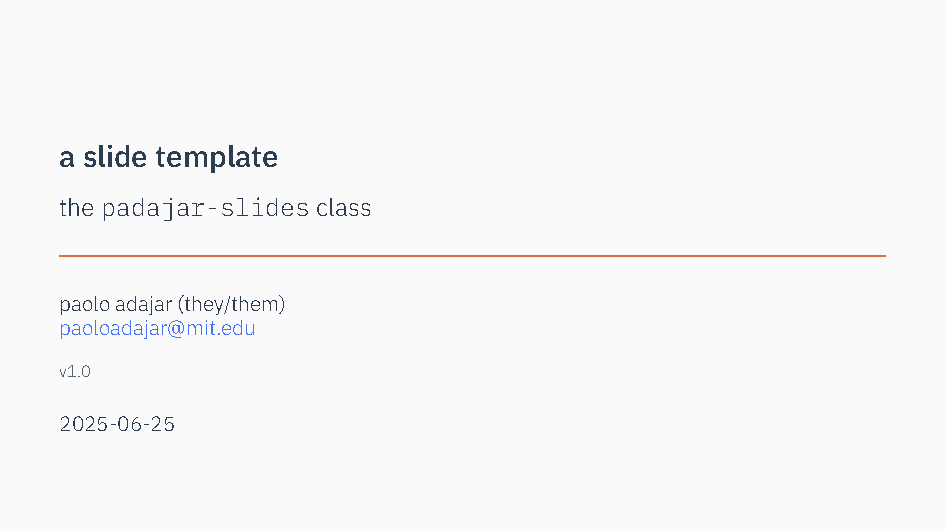
\includegraphics[width=0.49\textwidth,page=1]{slides/slides-example.pdf}
		\includegraphics[width=0.49\textwidth,page=4]{slides/slides-example.pdf}
		\includegraphics[width=0.49\textwidth,page=5]{slides/slides-example.pdf}
		\includegraphics[width=0.49\textwidth,page=6]{slides/slides-example.pdf}
		\end{center}
	\end{figure}

Key features include:
\begin{itemize}
	\item Navigation bubbles with section titles on the bottom of slides
	\item The \texttt{[sectionslides]} argument, which, when called, will add a navigation slide at the start of each section.
	\item \ttslash{graycitep}, which will cite bibliography items like \ttslash{citep} from the \texttt{natbib} package, but will insert citations into smaller, gray text.
	\item \ttslash{btLstHL}, which can highlight specific lines in an \texttt{lstlisting} environment by using the option	\texttt{linebackgroundcolor={\textbackslash btLstHL<overlay spec>\{range list\}}}
	\item A default 16:9 aspect ratio, the objectively correct aspect ratio for presentations.
\end{itemize}


\section{issues}

This set of files is \textit{far} from perfect right now. Some high-priority issues on my to-do list include:

\begin{itemize}
	\item Missing characters. I've done \href{https://tex.stackexchange.com/questions/739639/making-ibm-plex-math-thinner/}{some shenanigans} to make the math font thinner, and as a result, there are several missing math characters: \ttslash{epsilon}, \ttslash{varpi}, \ttslash{varrho}, \ttslash{nabla}, \ttslash{surd}, \ttslash{mapstochar}, \ttslash{lmoustache}, \ttslash{rmoustache}, \ttslash{arrowvert}, and \ttslash{Arrowvert}. The first is set to display as \ttslash{varepsilon} ($\eps$), which is what I primarily use anyways, and the last two are legacy and shouldn't pose much of an issue. These should all be manually set to other fonts, but because these don't see much use for me, I haven't found the best replacements yet. One I have already redefined is \ttslash{partial} ($\partial$), which is lifted from \TeX{} Gyre Schola; peek inside \texttt{padajar-defaults} to see how missing characters should be manually defined.
	\item Find a better solution for that pesky interaction between \texttt{float}s and \ttslash{tcolorbox}.
	\item Fix a few things I \textit{know} are bad \LaTeX{} coding:
	\begin{itemize}
		\item When the body text is sans-serif, the math text also becomes sans-serif. To change it back to serif, I use \ttslash{renewcommand\{\textbackslash text\}[1]\{\textbackslash oldtext\{\textbackslash rmfamily \#1\}}. Yuck.
		\item Yeah, yeah, I know I should fix \ttslash{epsilon} because \emph{some} people want to use it.
		\item Refactor the code, particularly looking for any repeated code and cleaning up the margins/parskip/etc. formatting; that in particular has become a bit of a jumble.
		\item Nice code for coloring specific rows/cells of a table? Perhaps something like \href{https://tex.stackexchange.com/questions/213301/efficiently-colouring-block-of-table-cells}{here}.
	\end{itemize}
\end{itemize}

\section{planned features}
These are features I'd like to add in the future, but aren't high priority for me at the moment.

\begin{itemize}
	\item Create the \texttt{padajar-paper} and \texttt{padajar-notes} class. I expect the former to be similar to \texttt{padajar-memo}, but with a few stylistic changes. The latter will probably be in a similar layout as well, but with functionality more akin to \href{https://web.stanford.edu/~lindrew/index.html}{lindrew}'s notes package.
	\item Make \ttslash{btLstHL} work outside of \texttt{beamer} classes (i.e., in documents).
	\item More common math shortcuts? I know there's plenty more I use.
	\item Add the \texttt{subfiles} package (pending research; some online seem to strongly prefer just using \ttslash{include} and \ttslash{includeonly}).
	\item A much closer look at all math symbols, finding alternatives for ones that I think have too much weight.
	\item Just a general look into compile time, and seeing if there are any ways to speed it up.
\end{itemize}

\section{unplanned features}

Conversely, here are some things that I explicitly \textit{don't} plan on doing with this set of classes.

\begin{itemize}
	\item Adding these to CTAN. I think it's incredibly unlikely that these see widespread usage, and probably isn't worth my time. I also think there's far too much idiosyncrasy in all of these formats for them to be used widely. But I guess if you think this has a broader interest, let me know?
	\item Letting fonts, by default, be something other than IBM Plex. I just like the aesthetic.
\end{itemize}

\appendix


\section{changelog}


\begin{tabular}{T p{\textwidth-1.75in}}
	1.0.0 (2025-03-30) & first creation of the memo, pset, and slides classes, each importing the default package  \\
	0.1.0 (2021-07-19) & initial creation of what would become these classes: a series of \LaTeX{} commands accessed with \ttslash{input\{paolo-pset.tex\}}
\end{tabular}


\section{installation instructions}

To use this package and set of classes:

\begin{enumerate}
	\item Download the following files:
	\begin{itemize}
		\item \texttt{padajar-defaults.sty}
		\item \texttt{padajar-memo.cls}
		\item \texttt{padajar-pset.cls}
		\item \texttt{padajar-slides.cls}
	\end{itemize}
	\item Place them into \textit{one} of the following places:
	\begin{itemize}
		\item The same folder as the \texttt{.tex} that you are trying to create. This will make it available for only that project.
		\item Add it to a local \TeX{} folder, where instructions will vary depending on your \TeX{} installation. This will make it available for all projects on your system.
	\end{itemize}
	\item Compile your document using XeLaTeX or LuaLaTeX (required due to \texttt{fontspec}).
\end{enumerate}

\section{license\label{license}}
Copyright \copyright{} 2021--\the\year{}, Paolo Adajar (\href{mailto:paoloadajar@mit.edu}{paoloadajar@mit.edu})

Permission is hereby granted, free of charge, to any person obtaining a copy of this software and associated documentation files (the “Software”), to deal in the Software without restriction, including without limitation the rights to use, copy, modify, merge, publish, distribute, sublicense, and/or sell copies of the Software, and to permit persons to whom the Software is furnished to do so, subject to the following conditions:

The above copyright notice and this permission notice shall be included in all copies or substantial portions of the Software.

THE SOFTWARE IS PROVIDED “AS IS”, WITHOUT WARRANTY OF ANY KIND, EXPRESS OR IMPLIED, INCLUDING BUT NOT LIMITED TO THE WARRANTIES OF MERCHANTABILITY, FITNESS FOR A PARTICULAR PURPOSE AND NONINFRINGEMENT. IN NO EVENT SHALL THE AUTHORS OR COPYRIGHT HOLDERS BE LIABLE FOR ANY CLAIM, DAMAGES OR OTHER LIABILITY, WHETHER IN AN ACTION OF CONTRACT, TORT OR OTHERWISE, ARISING FROM, OUT OF OR IN CONNECTION WITH THE SOFTWARE OR THE USE OR OTHER DEALINGS IN THE SOFTWARE.

\end{document}
